% =====================================================================
%  Resumo expandido - Aprendizado de Maquina Explicavel (XAI) - UFPR
%  Identificacao de Padroes de Dificuldade em Leitura e Escrita via XAI
%
%  Como compilar no Overleaf:
%    Menu > Compiler: pdfLaTeX  |  Main document: main.tex
%  Estrutura do projeto:
%    main.tex            -> este arquivo (texto do trabalho)
%    referencias.bib     -> referencias bibliograficas (BibTeX)
%    figuras/            -> logo da UFPR, graficos e diagrama (fluxo.tex)
%    codigo_figuras/     -> scripts Python que geram os graficos de figuras/
%
%  Todos os numeros vem dos scripts do repositorio
%  github.com/deborazanoello/xai_identificacao_de_dificuldades_de_leitura_e_escrita
%  O script codigo/conferir_numeros.py confere cada numero deste arquivo.
%  Comentarios marcados com  % CONFIRA  pedem revisao antes de submeter.
% =====================================================================
\documentclass[conference]{IEEEtran}
\IEEEoverridecommandlockouts

% ---------------------------------------------------------------- idioma
\usepackage[T1]{fontenc}
\usepackage[utf8]{inputenc}
\usepackage[brazilian]{babel}
\usepackage{icomma}            % virgula decimal em modo matematico: $0,91$

% ---------------------------------------------------------------- pacotes
\usepackage{cite}
\usepackage{amsmath,amssymb}
\usepackage{graphicx}
\usepackage{booktabs}
\usepackage{array}
\usepackage{xcolor}
\usepackage{tikz}
\usetikzlibrary{positioning,arrows.meta,fit,calc}
\usepackage{eso-pic}           % logo da UFPR no canto superior da 1a pagina
\usepackage{url}
\usepackage{balance}           % equilibra as colunas da ultima pagina
\usepackage[hidelinks]{hyperref}
\makeatletter
\g@addto@macro\UrlBreaks{\do\_}   % links longos quebram também no sublinhado
\makeatother

% ---------------------------------------------------------------- cores
\definecolor{corEscrita}{HTML}{2A78D6}   % mesmas cores dos graficos
\definecolor{corLeitura}{HTML}{EB6834}

% ---------------------------------------------------------------- atalhos
\newcommand{\RF}{Random Forest}
\newcommand{\Rdois}{R\textsuperscript{2}}

% ---------------------------------------------------------------- sem travessao
% O IEEEtran escreve "Resumo---" e "Index Terms---"; aqui o travessao vira dois-pontos.
\makeatletter
\def\abstract{\normalfont\@IEEEabskeysecsize\bfseries\textit{\abstractname}:\ \relax\@IEEEgobbleleadPARNLSP}
\def\IEEEkeywords{\normalfont\@IEEEabskeysecsize\bfseries\textit{\IEEEkeywordsname}:\ \relax\@IEEEgobbleleadPARNLSP}
\makeatother

% ---------------------------------------------------------------- logo UFPR
% Igual ao template: logo pequeno no canto superior direito da 1a pagina.
% Para mudar a posicao, ajuste os valores 0.75in (margem direita) e 0.30in (topo).
\AddToShipoutPictureFG*{%
  \AtPageUpperLeft{%
    \put(\LenToUnit{\paperwidth-0.75in-0.62in},\LenToUnit{-0.30in-0.393in}){%
      
\includegraphics[width=0.62in]{figuras/logo-ufpr.png}}}}

\begin{document}
% Controle do IEEEtran.bst, definido em referencias.bib: sem travessao para autores repetidos.
\bstctlcite{IEEEexample:BSTcontrol}

% =====================================================================
\title{Identificação de Padrões de Dificuldade em\\ Leitura e Escrita via XAI}

% CONFIRA: substitua pelos e-mails institucionais reais dos autores.
\author{%
\IEEEauthorblockN{Allysson Souza, Débora Zanoello, Marcelo Carvalho}
\IEEEauthorblockA{Orientador: Prof. Dr. Anderson Ara, DEST/LEG/UFPR\\
Disciplina de Aprendizado de Máquina Explicável\\
Universidade Federal do Paraná\\
Curitiba, Paraná, Brasil\\
\{email1,email2,email3\}@ufpr.br}}

\maketitle

% =====================================================================
\begin{abstract}
Investigamos se modelos interpretáveis por construção bastam para duas
previsões de um assistente proativo de leitura e escrita. A primeira é a
hesitação ao transcrever um texto, a partir do ritmo de digitação de 96
participantes da base KeyRecs, a mesma das atividades anteriores da disciplina.
A segunda usa uma base nova nesta etapa, pública e bem maior, o CompLex: a
dificuldade de 8.579 termos em contexto, tomada como aproximação dos termos que
o leitor tende a buscar. As duas bases passam pelo mesmo protocolo.
Comparamos regressão linear e logística, árvores podadas e EBM, modelos
interpretáveis, com Random Forest e XGBoost, modelos caixa-preta, em validação
cruzada. Na escrita, a regressão linear teve o menor erro, com RMSE de
0,031~s, sem diferença significativa para o Random Forest, $p = 0,33$. Na
leitura, o EBM igualou o Random Forest, com AUC de 0,919 nos dois. Em seguida,
aplicamos ao Random Forest sete métodos globais de explicabilidade: estatística
H de Friedman, decomposição funcional, importância por permutação, importância
por remoção ou LOFO, modelos substitutos globais, extração de regras e
protótipos e críticas. Os dois modelos são quase aditivos, e os efeitos
principais reproduzem de 93\% a 97\% da previsão; a árvore substituta e as
regras os resumem com fidelidade de 0,79 a 0,98. Com o mesmo protocolo de LOFO
nas duas bases, uma variável domina cada tarefa: retirar o tempo de voo na
senha aumenta o RMSE em 30\%, ou 10,4~ms, e retirar a frequência da palavra
reduz a AUC em 16,7 pontos. Quando há uma variável substituta, colocada de
propósito na escrita e natural na leitura, essa importância se divide entre as
duas. Na leitura, os maiores erros do modelo são palavras comuns que os leitores
acharam difíceis, cujo sentido depende do contexto.
\end{abstract}

\begin{IEEEkeywords}
explicabilidade, interpretabilidade, aprendizado de máquina, XAI, dinâmica de
digitação, complexidade lexical
\end{IEEEkeywords}

% =====================================================================
\section{Introdução}

Dificuldades de leitura e de escrita aparecem em momentos concretos, como uma
pausa longa antes de digitar uma palavra ou um termo que obriga o leitor a
interromper a leitura para buscar seu significado. Um assistente pessoal
proativo poderia antecipar esses momentos e oferecer ajuda antes que o usuário
peça. Para isso, são necessárias duas previsões: \emph{quando} a pessoa tende a
hesitar ao escrever e \emph{quais} termos de um texto ela tende a buscar.

Nesse cenário, a explicabilidade não é um acessório. Um assistente que intervém
sem que se saiba por quê dificilmente ganha a confiança do usuário, e um modelo
que acerta pelos motivos errados pode reproduzir padrões espúrios. A literatura
de aprendizado de máquina interpretável distingue modelos interpretáveis por
construção, cuja estrutura já é a explicação, de modelos caixa-preta explicados
por métodos pós-hoc~\cite{molnar2022,doshivelez2017}. Rudin~\cite{rudin2019stop}
argumenta que, quando um modelo interpretável alcança o desempenho da
caixa-preta, ele deve ser preferido. Os métodos pós-hoc, tanto locais, como
LIME~\cite{ribeiro2016lime} e SHAP~\cite{lundberg2017shap}, quanto globais,
continuam úteis para verificar o que a caixa-preta aprendeu e se isso coincide
com o que o modelo interpretável mostra.

Este trabalho continua as Atividades 02 a 04 da disciplina, que usaram apenas
a base pública KeyRecs~\cite{dias2023keyrecs,dias2023keyrecsdata}, de dinâmica
de digitação, para a previsão na escrita. Nesta etapa, o trabalho evoluiu em
três frentes. Primeiro, introduzimos uma base nova, o
CompLex~\cite{shardlow2020complex}, de complexidade lexical, também pública e
bem maior, com 8.579 termos contra 96 participantes, para a previsão na
leitura. Segundo, aplicamos às duas bases o mesmo protocolo, com a mesma
comparação entre modelos, o mesmo LOFO e outros seis métodos globais, o que
permite comparar as duas tarefas lado a lado. Terceiro, revisamos a base da
escrita e corrigimos o cálculo do tempo de voo na senha. Todo o material, das
atividades anteriores a esta etapa, foi consolidado em um único repositório
público, com uma cópia de cada base.

O \textbf{objetivo} é verificar se modelos interpretáveis por construção bastam
para as duas tarefas e usar métodos globais de XAI para entender o que a
caixa-preta aprendeu. Buscamos responder se o modelo interpretável alcança a
caixa-preta, quanto da previsão vem de efeitos isolados e quanto vem de
interações, quais variáveis concentram o efeito, se é possível resumir a
caixa-preta em algo legível com alta fidelidade, quais casos o modelo
representa mal e o que se repete e o que muda de uma base para a outra.

\textbf{Enquadramento ético.} Os modelos usam padrões de digitação e
características das palavras. Eles não fazem diagnóstico de nenhuma condição e
não rotulam pessoas; o objetivo é decidir quando e onde oferecer ajuda.

% =====================================================================
\section{Dados}

A Tabela~\ref{tab:bases} resume as duas bases. Em ambas, as variáveis foram
escolhidas para serem compreensíveis por um usuário do assistente.

\begin{table}[!t]
\caption{Resumo das duas bases públicas: a KeyRecs vem das atividades anteriores, e o CompLex entrou nesta etapa.}
\label{tab:bases}
\centering
\footnotesize
\setlength{\tabcolsep}{4pt}
\begin{tabular}{@{}>{\raggedright\arraybackslash}p{1.55cm}
                >{\raggedright\arraybackslash}p{3.05cm}
                >{\raggedright\arraybackslash}p{3.05cm}@{}}
\toprule
 & \textbf{Escrita} & \textbf{Leitura} \\
\midrule
Base        & KeyRecs~\cite{dias2023keyrecs,dias2023keyrecsdata} & CompLex~\cite{shardlow2020complex} \\
No trabalho & Atividades 02 a 04 e esta etapa & Nova nesta etapa \\
Pergunta    & O ritmo de digitação na senha antecipa a hesitação ao transcrever um texto?
            & Quais termos do texto o leitor tende a buscar? \\
Unidade     & 96 participantes, após os filtros
            & 8.579 termos em contexto, em inglês \\
Alvo        & Hesitação: mediana do tempo de voo na transcrição, em s
            & Termo difícil: complexidade $\geq 0,5$, em 9,7\% dos termos \\
Variáveis   & 7: tempo de voo, pressionamento, CV do tempo total e ganho com
              a prática, na senha; idade, gênero, lateralidade
            & 8: frequência no idioma, comprimento, sílabas, sigla, nome próprio,
              tamanho da frase, posição, forma em português \\
Correlação  & $r = 0,73$ entre voo na senha e hesitação
            & $r = -0,63$ entre frequência e complexidade \\
\bottomrule
\end{tabular}
\end{table}

\subsection{Escrita: KeyRecs}

A KeyRecs~\cite{dias2023keyrecs,dias2023keyrecsdata} é uma base pública de
dinâmica de digitação, com licença CC BY 4.0, em que cada participante fez dois
exercícios: redigitar uma senha fixa, cerca de 100 vezes em cada uma de duas
sessões, e transcrever um texto. Ela registra os tempos de cada tecla e
informações demográficas dos participantes. Após os filtros, restaram 96
participantes, 19.767 repetições da senha e 559.514 pares de teclas no texto
livre. A unidade de análise é o participante.

A variável resposta é a \emph{hesitação}, definida como a mediana do tempo de
voo, isto é, da pausa entre teclas consecutivas, durante a transcrição, em
segundos. As sete variáveis explicativas vêm do exercício da senha e do perfil
do participante. Da senha saem quatro medidas motoras: o tempo de voo, mediana
da pausa entre soltar uma tecla e apertar a seguinte; o tempo de
pressionamento, mediana do tempo em que a tecla fica pressionada, o
\emph{dwell}; a consistência, medida pelo coeficiente de variação, ou CV, do
tempo total da senha entre as repetições; e o ganho com a prática, a queda
relativa da mediana do tempo total da primeira para a segunda sessão. Do perfil
entram idade, gênero e lateralidade. O tempo de voo na senha já tem correlação
de $r = 0,73$ com a hesitação. O tempo total da senha, medido entre soltar a
primeira tecla e apertar a última, tem correlação de 0,78 com o tempo de voo e
foi excluído do modelo por colinearidade; ele volta na
Seção~\ref{sec:importancia}, em um experimento sobre variáveis substitutas.

\emph{Conferência da base.} Rodado de novo sobre os arquivos públicos da
KeyRecs, o código de construção da tabela reproduz exatamente a tabela usada
nas Atividades 02 a 04. A limpeza descarta pausas e pressionamentos acima de
10~s e repetições da senha acima de 60~s, o que elimina as repetições
corrompidas da base, como um tempo total negativo, e exige hesitação positiva.
Por isso ficaram de fora três participantes, p043, p071 e p078, com hesitação
menor ou igual a zero, típica de quem digita sobrepondo teclas. No arquivo da
senha, os rótulos das colunas de pares de teclas estão trocados em relação às
definições usuais, o que se verifica pelas identidades entre os tempos, válidas
em todas as linhas; no texto livre, estão corretos. Nas Atividades 02 a 04, o
tempo de voo da senha foi calculado pelo rótulo e equivalia à pausa real
somada à diferença entre os pressionamentos da segunda e da primeira tecla. As
duas versões têm correlação de 0,994, e a diferença mediana entre elas é de
4~ms. Neste trabalho, o tempo de voo foi recalculado com a pausa real, e todos
os resultados da escrita usam essa versão; com a versão anterior, as
conclusões são as mesmas, como mostra a Seção~\ref{sec:importancia}.

\subsection{Leitura: CompLex}

O CompLex~\cite{shardlow2020complex} reúne termos em inglês, cada um dentro da
frase em que aparece, anotados por leitores em uma escala de complexidade, em
textos da Bíblia, artigos biomédicos e atas do Parlamento Europeu. Usamos os
8.579 termos de uma palavra das partes de treino e de teste da versão pública,
disponível no GitHub com licença CC BY. A variável resposta é binária: o termo é
considerado \emph{difícil} quando sua complexidade média é pelo menos 0,5, o
que ocorre em 9,7\% dos casos. Esse rótulo é usado como aproximação do termo
que o leitor buscaria.

As oito variáveis explicativas descrevem a palavra e o contexto e foram
calculadas por nós a partir do texto. A frequência no idioma está na escala
Zipf, o logaritmo da frequência por bilhão de palavras, obtida da biblioteca
wordfreq~\cite{speer2022wordfreq}. As demais são o comprimento, em letras; o
número de sílabas; a sigla, quando o termo tem duas ou mais maiúsculas ou
maiúscula fora da primeira letra; o nome próprio, quando tem inicial maiúscula
fora do início da frase; o tamanho da frase, em palavras; a posição relativa do
termo na frase; e a forma em português, igual a 1 quando a mesma grafia também
é frequente em português, com Zipf $\geq 3$. A frequência tem correlação de
$r = -0,63$ com a complexidade: quanto mais rara a palavra, mais complexa ela
tende a ser.

% =====================================================================
\section{Metodologia}

A Fig.~\ref{fig:fluxo} resume o fluxo da análise. Nas duas tarefas, modelos
interpretáveis por construção são comparados com modelos caixa-preta, e sete
métodos globais, organizados em quatro perguntas, são aplicados ao \RF{}. Na
escrita, a comparação de modelos segue as Atividades 02 e 03, e o LOFO segue a
Atividade 04, todos refeitos aqui com o tempo de voo corrigido. A leitura foi
analisada aqui pela primeira vez, com o mesmo protocolo.

\begin{figure*}[!t]
\centering
% =====================================================================
%  Fig. 1 - Fluxo da analise (TikZ). Incluido em main.tex com \input.
%  Edite os textos diretamente aqui; as cores estao definidas em main.tex
%  (corEscrita, corLeitura).
% =====================================================================
\begin{tikzpicture}[
    font=\footnotesize,
    >={Stealth[length=2mm]},
    caixa/.style={draw=black!55, rounded corners=2pt, align=center,
                  inner sep=3pt, line width=0.5pt},
    base/.style={caixa, text width=2.9cm, minimum height=1.25cm},
    meio/.style={caixa, text width=3.1cm, fill=black!4},
    metodo/.style={caixa, text width=4.45cm, minimum height=1.25cm,
                   fill=white, align=left},
    seta/.style={->, line width=0.6pt, draw=black!70},
    rotulo/.style={font=\scriptsize\bfseries, text=black!65}
]
% ---------------- bases de dados
\node[base, fill=corEscrita!10, draw=corEscrita] (keyrecs)
  {\textbf{Escrita · KeyRecs}\\ 96 participantes\\ alvo: hesitação, em s};
\node[base, fill=corLeitura!10, draw=corLeitura, below=0.35cm of keyrecs] (complex)
  {\textbf{Leitura · CompLex}\\ 8.579 termos em contexto\\ alvo: termo difícil};

% ---------------- modelos preditivos
\node[meio, right=0.75cm of $(keyrecs.east)!0.5!(complex.east)$, anchor=west,
      minimum height=2.85cm] (ativ)
  {\textbf{Modelo preditivo}\\[2pt]
   Interpretável por construção:\\ regressão, árvore, EBM\\[1pt]
   $\times$\\[1pt]
   Caixa-preta:\\ Random Forest, XGBoost\\[2pt]
   validação cruzada $5\times10$};

% ---------------- 4 perguntas, 7 metodos globais
\node[metodo, right=0.8cm of ativ.north east, anchor=north west, yshift=0.0cm] (m12)
  {\textbf{Como as variáveis se combinam?}\\
   \textcircled{\scriptsize 1} H de Friedman\\
   \textcircled{\scriptsize 2} Decomposição funcional};
\node[metodo, right=0.2cm of m12] (m34)
  {\textbf{Quais variáveis importam?}\\
   \textcircled{\scriptsize 3} Permutação\\
   \textcircled{\scriptsize 4} Remoção, LOFO};
\node[metodo, below=0.35cm of m12] (m56)
  {\textbf{Como resumir o forest?}\\
   \textcircled{\scriptsize 5} Substitutos globais\\
   \textcircled{\scriptsize 6} Extração de regras};
\node[metodo, below=0.35cm of m34] (m7)
  {\textbf{Quais casos são atípicos?}\\
   \textcircled{\scriptsize 7} Protótipos e críticas,\\
   \phantom{x}MMD-critic};

\node[draw=black!40, dashed, rounded corners=3pt, inner sep=4pt,
      fit=(m12)(m34)(m56)(m7)] (a4) {};
\node[rotulo, anchor=south west] at (a4.north west)
  {MÉTODOS GLOBAIS APLICADOS AO RANDOM FOREST DE CADA TAREFA};

% ---------------- setas
\draw[seta] (keyrecs.east) -- ++(0.35,0) |- (ativ.west);
\draw[seta] (complex.east) -- ++(0.35,0) |- (ativ.west);
\draw[seta] (ativ.east) -- (a4.west |- ativ.east);
\end{tikzpicture}

\caption{Fluxo da análise. As duas bases passam pelo mesmo protocolo: a
comparação entre modelos interpretáveis por construção e caixa-preta e, em
seguida, sete métodos globais, agrupados em quatro perguntas, aplicados ao
Random Forest de cada tarefa.}
\label{fig:fluxo}
\end{figure*}

\subsection{Modelo preditivo}

\emph{Escrita, uma regressão.} Ajustamos uma linha de base que prevê a mediana,
uma regressão linear, uma árvore de decisão podada e um
\RF{}~\cite{breiman2001rf} com 500 árvores, ou 300 no LOFO. O tamanho mínimo
das folhas e a fração de variáveis sorteadas em cada divisão da floresta foram
escolhidos por busca em grade, com validação cruzada interna em 70\% dos dados;
a árvore foi podada pelo custo de complexidade, com a regra do 1-EP. O
desempenho foi estimado por validação cruzada com 5 dobras repetida 10 vezes,
isto é, 50 dobras, com RMSE e erro absoluto médio, o MAE, em segundos, e
\Rdois{}. As diferenças entre modelos foram avaliadas pelo teste $t$ corrigido
para validação cruzada~\cite{nadeau2003inference}, que leva em conta a
sobreposição entre os conjuntos de treino, com razão teste/treino de 0,25. As
análises usaram o scikit-learn~\cite{pedregosa2011sklearn}.

\emph{Leitura, uma classificação.} Ajustamos uma regra fixa baseada na raridade
da palavra, uma regressão logística, uma árvore podada, um
EBM~\cite{lou2013ga2m,nori2019interpretml}, um \RF{} e um
XGBoost~\cite{chen2016xgboost}. Como a mesma palavra pode aparecer em várias
frases, a validação cruzada foi agrupada por palavra: um termo nunca aparece ao
mesmo tempo no treino e no teste. Usamos quatro métricas. A AUC mede a
ordenação geral. A \emph{precisão nos 10\%} é a proporção de termos difíceis
entre os 10\% de termos com maior probabilidade prevista e corresponde ao uso
pretendido, em que o assistente sugere poucos termos e eles devem estar certos.
A precisão média, área sob a curva de precisão e revocação, é mais adequada a
uma classe rara: o valor de um modelo sem informação é a própria proporção de
difíceis, 0,097. O escore de Brier, erro quadrático médio da probabilidade
prevista, mede a calibração; prever sempre a proporção de difíceis dá 0,088.
Para olhar a calibração mais de perto, usamos as previsões fora da amostra de
uma validação cruzada agrupada de 5 dobras e calculamos o erro de calibração
esperado, a diferença média entre a probabilidade prevista e a proporção
observada em 10 faixas de probabilidade, e a inclinação de calibração, que vale
1 quando as probabilidades não precisam ser esticadas nem comprimidas.
Os hiperparâmetros foram escolhidos uma única vez, em 70\% das palavras: \RF{}
com 500 árvores, fração de 0,3 das variáveis em cada divisão e folhas com pelo
menos 10 termos; árvore com 15 folhas, pela regra do 1-EP; XGBoost com 300
árvores de profundidade 3 e taxa de aprendizado de 0,03; EBM sem interações; e
regressão logística com as variáveis padronizadas. O desempenho foi estimado em
$5 \times 10$ dobras.

O EBM, ou \emph{Explainable Boosting Machine}, é um modelo aditivo generalizado
ajustado por \emph{boosting}: a previsão é a soma de uma função de forma por
variável, que pode ser lida diretamente em um gráfico~\cite{nori2019interpretml}.
Na escrita, a Atividade 03 também explicou as previsões localmente, com
LIME~\cite{ribeiro2016lime} e SHAP~\cite{lundberg2017shap}, ainda com a versão
anterior do tempo de voo.

\subsection{Métodos de explicabilidade}

Os sete métodos a seguir foram aplicados ao \RF{} de cada tarefa, tratado como
o modelo caixa-preta a ser explicado. Para H, decomposição funcional,
substitutos e regras, a floresta foi treinada em 70\% dos dados, ou 70\% das
palavras na leitura, e avaliada nos 30\% restantes. Na leitura, a previsão
explicada é a probabilidade de o termo ser difícil.

\emph{Estatística H de Friedman.} Mede quanto da variação da previsão se deve
a interações~\cite{friedman2008rulefit}. Para um par de variáveis $j$ e $k$,
com funções de dependência parcial centradas $PD$,
\begin{equation}
H^2_{jk} = \frac{\sum_{i=1}^{n}\left[PD^{(i)}_{jk} - PD^{(i)}_{j} - PD^{(i)}_{k}\right]^2}{\sum_{i=1}^{n} \left(PD^{(i)}_{jk}\right)^2},
\end{equation}
em que $PD^{(i)}_{jk}$ é a dependência parcial avaliada na observação $i$. A
versão $H_j$ mede a interação de uma variável com todas as outras. O valor 0
indica nenhuma interação, e o valor 1 indica que todo o efeito vem de
interações. Na escrita, estimamos a incerteza do H por bootstrap, com 100
reamostragens dos participantes de treino e a floresta treinada de novo em cada
uma.

\emph{Decomposição funcional.} Escreve a previsão como
\begin{equation}
\hat f(\mathbf{x}) = f_0 + \sum_{j} f_j(x_j) + \sum_{j<k} f_{jk}(x_j,x_k) + \cdots,
\end{equation}
isto é, constante, efeitos principais e
interações~\cite{hooker2004additive,molnar2022}. Medimos o \Rdois{} entre a
previsão completa e a soma da constante com os efeitos principais. Se esse
valor é próximo de 1, o modelo é quase aditivo.

\emph{Importância por permutação.} Com o modelo já treinado, os valores de uma
variável são embaralhados no conjunto de teste, e mede-se quanto o desempenho
piora~\cite{breiman2001rf,fisher2019all}. Calculamos a permutação nas mesmas 50
dobras do LOFO, com o teste $t$ corrigido.

\emph{Importância por remoção, o LOFO.} Mede quanto o modelo perde quando não
pode usar uma variável~\cite{lei2018loco,williamson2023general}:
\begin{equation}
\mathrm{LOFO}_j = \mathbb{E}\big[L\big(Y, \hat f_{-j}(X_{-j})\big)\big] - \mathbb{E}\big[L\big(Y, \hat f(X)\big)\big],
\end{equation}
em que $\hat f_{-j}$ é o mesmo algoritmo treinado de novo sem $X_j$ e $L$ é a
perda fora da amostra: o RMSE, na escrita, e a queda da AUC, na leitura. Em
cada uma das 50 dobras, o modelo é ajustado com todas as variáveis e sem cada
uma delas, com os mesmos hiperparâmetros. Como as dobras são as mesmas para
todas as variáveis, as diferenças são pareadas, e a significância é avaliada
pelo teste $t$ corrigido~\cite{nadeau2003inference}. Como cada LOFO testa
várias variáveis ao mesmo tempo, sete na escrita e oito na leitura, também
ajustamos os valores $p$ pela correção de Holm~\cite{holm1979simple}, que
controla a chance de pelo menos um falso positivo. Diferente da permutação, o LOFO nunca mostra ao modelo
combinações artificiais de valores~\cite{hooker2021permutation} e mede a
contribuição única da variável: se outra variável carrega a mesma informação, a
remoção quase não prejudica o modelo. A concordância entre as ordenações de
importância do LOFO e da permutação foi medida pela correlação de Spearman,
$\rho$, com intervalo de 95\% por bootstrap das 10 repetições da validação
cruzada.

Na escrita, aprofundamos o LOFO com testes complementares, todos nas mesmas 50
dobras e com os mesmos hiperparâmetros: a \emph{estabilidade} do ranking, em
cinco partições com sementes diferentes, de $5 \times 2$ dobras cada, e com
dez sementes da floresta em dez dobras fixas; a \emph{dependência do
algoritmo}, com o LOFO da regressão linear; a \emph{dependência entre
variáveis}, devolvendo ao modelo o tempo total da senha e removendo também o
par voo e tempo total e blocos de variáveis, as demográficas e as motoras; a
\emph{suficiência}, com a floresta ajustada a uma variável só; a
\emph{permutação nas mesmas dobras}, com 20 embaralhamentos por dobra;
\emph{outras perdas}, o MAE e o RMSE nos 25\% de maior hesitação; \emph{outros
alvos}, as taxas de pausas longas e de revisão no texto livre; e a
sensibilidade a \emph{hiperparâmetros reajustados} sem cada variável e à
\emph{versão da tabela}. Na leitura, repetimos a estabilidade em 10 repetições,
os blocos de variáveis correlacionadas e a suficiência.

\emph{Modelos substitutos globais.} Um modelo interpretável, aqui uma árvore de
profundidade 3 e uma regressão linear, é treinado para imitar as previsões do
\RF{}~\cite{craven1996trepan,molnar2022}. A \emph{fidelidade} é o \Rdois{}
entre as previsões do substituto e as do \RF{} no conjunto de teste.

\emph{Extração global de regras.} Os caminhos das árvores do \RF{} são
convertidos em regras do tipo SE~\ldots{} ENTÃO, e uma lista curta é montada
escolhendo, a cada passo, a regra cujas previsões do \RF{} são mais
homogêneas, em linha com abordagens como RuleFit e
inTrees~\cite{friedman2008rulefit,deng2019intrees}. A lista termina com uma
regra SENÃO, e sua fidelidade também é medida pelo \Rdois{} no teste.

\emph{Protótipos e críticas.} O MMD-critic~\cite{kim2016mmdcritic} escolhe
protótipos, os casos que melhor representam a distribuição dos dados, e
críticas, os casos atípicos que os protótipos representam mal. Comparar o
comportamento do modelo nos dois grupos mostra se ele falha justamente onde os
dados fogem do padrão.

% =====================================================================
\section{Resultados}

\subsection{Desempenho preditivo}

As Tabelas~\ref{tab:escrita} e~\ref{tab:leitura} apresentam o desempenho dos
modelos. Nas duas tarefas, o modelo interpretável por construção alcançou a
caixa-preta. Na escrita, a regressão linear teve o menor erro, com RMSE de
0,0314~s, MAE de 0,0250~s e \Rdois{} de 0,42, e a diferença para o \RF{} não
foi significativa, $p = 0,33$. A árvore podada fez um único corte, em tempo de
voo na senha acima de 0,138~s, e já explicou 30\% da variação. A linha de base
teve \Rdois{} negativo, o que é esperado para uma previsão constante avaliada
fora da amostra.

\begin{table}[!t]
\caption{Escrita, KeyRecs: desempenho em validação cruzada $5\times10$.}
\label{tab:escrita}
\centering
\footnotesize
\setlength{\tabcolsep}{5pt}
\begin{tabular}{@{}lccc@{}}
\toprule
\textbf{Modelo} & \textbf{RMSE, s} & \textbf{MAE, s} & \textbf{\Rdois} \\
\midrule
Linha de base, a mediana       & 0,0450 & 0,0360 & $-0,10$ \\
Regressão linear$^\dagger$$^\star$ & \textbf{0,0314} & \textbf{0,0250} & \textbf{0,42} \\
Árvore podada$^\dagger$, 1 corte & 0,0351 & 0,0284 & 0,30 \\
\RF                            & 0,0342 & 0,0274 & 0,34 \\
\bottomrule
\multicolumn{4}{@{}p{0.95\columnwidth}@{}}{\scriptsize $^\dagger$Interpretável
por construção. $^\star$Modelo escolhido. \RF{} contra regressão linear:
$p = 0,33$ no teste $t$ corrigido para validação
cruzada~\cite{nadeau2003inference}.}
\end{tabular}
\end{table}

\begin{table}[!t]
\caption{Leitura, CompLex: desempenho em validação cruzada $5\times10$ agrupada por palavra.}
\label{tab:leitura}
\centering
\footnotesize
\setlength{\tabcolsep}{4.5pt}
\begin{tabular}{@{}lcccc@{}}
\toprule
\textbf{Modelo} & \textbf{AUC} & \textbf{Prec. 10\%} & \textbf{Prec. média} & \textbf{Brier} \\
\midrule
Regra das palavras raras$^\dagger$ & 0,849 & 0,382 & 0,356 & \\
Regressão logística$^\dagger$      & 0,914 & \textbf{0,506} & 0,520 & 0,062 \\
Árvore podada$^\dagger$, 15 folhas & 0,902 & 0,446 & 0,467 & 0,063 \\
EBM$^\dagger$$^\star$              & 0,919 & 0,496 & 0,534 & 0,061 \\
\RF                                & 0,919 & 0,491 & 0,530 & \textbf{0,060} \\
XGBoost                            & \textbf{0,922} & 0,500 & \textbf{0,539} & \textbf{0,060} \\
\bottomrule
\multicolumn{5}{@{}p{0.95\columnwidth}@{}}{\scriptsize $^\dagger$Interpretável
por construção. $^\star$Modelo escolhido. Em negrito, o melhor valor de cada
coluna; no Brier, menor é melhor. A regra não dá probabilidade e não tem Brier.
Sem informação, a precisão média seria 0,097 e o Brier, 0,088. AUC do \RF{}
contra EBM: $p = 0,82$; contra regressão logística: $p = 0,18$; contra
XGBoost: $p = 0,12$.}
\end{tabular}
\end{table}

Na leitura, o EBM igualou o \RF{} em AUC, 0,919 nos dois, com $p = 0,82$, e
também na precisão nos 10\%, com 0,496 contra 0,491, na precisão média, com
0,534 contra 0,530, e no Brier, com 0,061 contra 0,060. A regressão logística
ficou próxima, com AUC de 0,914 e $p = 0,18$, e teve a maior precisão nos 10\%,
0,506. O XGBoost teve a maior AUC, 0,922, sem diferença significativa para o
\RF{}, $p = 0,12$, nem para o EBM, $p = 0,10$; só superou a regressão
logística, por 0,008, no limite da significância, $p = 0,05$. Na precisão média
e no Brier, nenhuma diferença entre esses quatro modelos foi significativa, com
$p \geq 0,06$. A árvore podada ficou abaixo do EBM, com $p = 0,02$ na AUC. A
regra das palavras raras, que usa apenas a frequência, já alcançou AUC de 0,849
e precisão média de 0,356, quase quatro vezes o valor de um modelo sem
informação. A calibração confirma o Brier: o erro de calibração esperado foi de
0,009 no EBM e no \RF{} e de 0,012 na regressão logística. A inclinação de
calibração foi de 0,99 no EBM e na regressão logística, próxima do ideal, e de
1,16 no \RF{}, cujas probabilidades ficam um pouco menos extremas do que
deveriam.

Na escrita, as explicações locais da Atividade 03 também apontaram um degrau no
tempo de voo perto de 0,14~s, e LIME e SHAP concordaram sobre a variável
principal em 90\% dos 29 participantes de teste.

\subsection{Como as variáveis se combinam}

A Tabela~\ref{tab:sintese} sintetiza os resultados dos sete métodos globais,
detalhados nesta subseção e nas seguintes. Na escrita, as variáveis com mais
interação foram o CV do tempo total e o tempo de voo, com $H = 0,17$ e 0,16, e
o único par com interação foi justamente esse, com $H = 0,17$; nas demais
variáveis, $H$ ficou abaixo de 0,01. Esses valores são incertos: no bootstrap
dos participantes de treino, o intervalo de 95\% do H do tempo de voo foi de
0,02 a 0,25. Na leitura, a variável com mais interação
foi a frequência, com $H = 0,26$, seguida do comprimento, com $H = 0,21$. Os
maiores $H$ por par na leitura, de até 0,54, entre sílabas e forma em
português, aparecem entre variáveis de efeito quase nulo, em que o denominador
da estatística é muito pequeno, e não devem ser interpretados. Entre os pares
com efeito relevante, o mais forte foi comprimento e sigla, com $H = 0,27$.

A decomposição funcional mostrou que os efeitos principais, sozinhos,
reproduzem a previsão do \RF{} com \Rdois{} de 0,97 na escrita e de 0,93 na
leitura; as interações respondem por 3\% e 7\%, respectivamente. Os maiores
componentes foram o tempo de voo, com 94\% da variância dos efeitos principais,
e o CV do tempo total, com 6\%, na escrita, e a frequência, com 69\%, a sigla,
com 19\%, e o comprimento, com 10\%, na leitura. Os dois modelos são, portanto,
quase aditivos, e as interações que existem envolvem as variáveis principais de
cada tarefa. Isso explica por que um modelo aditivo interpretável, como a
regressão ou o EBM, perde pouco em relação ao \RF{}.

\subsection{Quais variáveis importam}
\label{sec:importancia}

Na escrita, pela permutação nas mesmas 50 dobras do LOFO, só o tempo de voo
piora o modelo de forma distinguível de zero quando embaralhado, em 17,4~ms,
com $p < 0,001$; o CV do tempo total vem em segundo, com 0,8~ms e $p = 0,14$, e
as outras 5 variáveis ficam em torno de zero. Na leitura, pioram o modelo
sobretudo a frequência, em 29,1 pontos de AUC multiplicada por 100, o
comprimento, em 2,4, e a sigla, em 2,3. Nome próprio, tamanho da frase e forma
em português têm efeitos abaixo de 0,25 ponto, embora distinguíveis de zero, e
sílabas e posição não diferem de zero.

\emph{LOFO na escrita.} A Tabela~\ref{tab:lofo} e a Fig.~\ref{fig:lofo}a
mostram o LOFO do \RF{} no KeyRecs. Nesta análise, a floresta teve RMSE de
34,6~ms, contra 45,2~ms da previsão pela mediana; a pequena diferença em
relação à Tabela~\ref{tab:escrita} vem de a floresta do LOFO ter 300 árvores,
e não 500. Só o tempo de voo carrega informação única: sem ele, o RMSE sobe
10,4~ms, de 34,6 para 45,0~ms, uma piora de 30\% observada em 96\% das 50
dobras, com $p < 0,001$, ou $p = 0,004$ após a correção de Holm. O CV do tempo
total vem em segundo, com +0,52~ms, um efeito pequeno e incerto, com
$p = 0,33$. As demais variáveis ficam em torno de zero; pressionamento, idade e
ganho com a prática têm LOFO levemente negativo, isto é, a floresta generaliza
um pouco melhor sem elas.

\begin{table}[!t]
\caption{LOFO do Random Forest na escrita, KeyRecs: aumento do RMSE, em ms, ao remover cada variável.}
\label{tab:lofo}
\centering
\footnotesize
\setlength{\tabcolsep}{2.6pt}
\begin{tabular}{@{}lrrcccc@{}}
\toprule
\textbf{Variável} & \textbf{LOFO} & \textbf{dp} & \textbf{$>0$} & $\boldsymbol{p}$ & $\boldsymbol{p}$ \textbf{Holm} & \textbf{Posição$^\ast$} \\
\midrule
Tempo de voo        & $+10,36$ & 5,38 & 96\% & $<0,001$ & 0,004 & 1º em 5/5 \\
CV do tempo total   & $+0,52$  & 1,02 & 78\% & 0,33     & 1     & 2º em 5/5 \\
Lateralidade        & $0,00$   & 0,00 & 36\% & 0,61     & 1     & 3º a 5º \\
Gênero              & $-0,02$  & 0,07 & 46\% & 0,59     & 1     & 4º a 5º \\
Ganho com a prática & $-0,04$  & 0,11 & 44\% & 0,52     & 1     & 3º a 7º \\
Idade               & $-0,04$  & 0,12 & 44\% & 0,50     & 1     & 3º a 6º \\
Pressionamento      & $-0,09$  & 0,17 & 32\% & 0,31     & 1     & 6º a 7º \\
\bottomrule
\multicolumn{7}{@{}p{0.97\columnwidth}@{}}{\scriptsize dp: desvio-padrão entre as
50 dobras. $>0$: dobras em que o erro piorou. $p$: teste $t$
corrigido~\cite{nadeau2003inference}; $p$ Holm:
ajustado para as 7 comparações. $^\ast$Posição no ranking em 5 partições com
sementes diferentes, de $5\times2$ dobras cada.}
\end{tabular}
\end{table}

\begin{figure*}[!t]
\centering
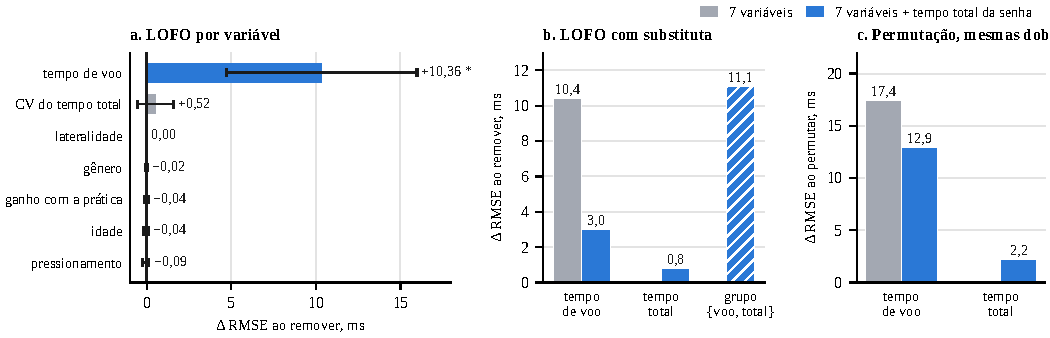
\includegraphics[width=\textwidth]{figuras/lofo_keyrecs.pdf}
\caption{LOFO na escrita, KeyRecs. a. Aumento do RMSE do Random Forest ao
remover cada variável, com intervalo de 95\% corrigido para a dependência entre
as 50 dobras~\cite{nadeau2003inference}; $^\ast p < 0,05$. b. Com o tempo total
da senha no modelo, a importância do tempo de voo se divide entre as duas
variáveis, mas o grupo formado pelas duas recupera a perda. c. Nas mesmas
dobras, a importância por permutação do tempo de voo, no modelo já treinado,
cai bem menos, $-26\%$.}
\label{fig:lofo}
\end{figure*}

\emph{Estabilidade.} Treinar o modelo de novo adiciona ruído: o desvio-padrão do
LOFO do tempo de voo entre as dobras, de 5,38~ms, é cerca de metade da média.
Mesmo assim, nas cinco partições com sementes diferentes, o tempo de voo ficou
em 1º lugar e o CV do tempo total em 2º em todas; da 3ª posição para baixo, a
ordem muda a cada partição e não deve ser interpretada.

\emph{Dependência do algoritmo.} Com a regressão linear, nas mesmas 50 dobras e
com RMSE de 31,8~ms, o tempo de voo pesa ainda mais: +12,8~ms, ou 40\% do RMSE.
Nenhuma outra variável difere de zero.

\emph{Variável substituta.} Quando o tempo total da senha volta ao modelo, o
LOFO do tempo de voo cai de 10,4 para 3,0~ms, uma perda de 71\%, e deixa de ser
significativo, com $p = 0,06$; o do tempo total fica em 0,8~ms. Cada uma cobre
a outra, como mostra a Fig.~\ref{fig:lofo}b. Removidas juntas, como grupo, a
perda volta a 11,1~ms. Já a permutação, nas mesmas 50 dobras, cai bem menos: de
17,4 para 12,9~ms, uma queda pareada de 4,5~ms, com intervalo de 95\% de 2,2 a
6,8~ms, ou $-26\%$, e o tempo total passa a 2,2~ms, como na
Fig.~\ref{fig:lofo}c. O modelo treinado continua apoiado no tempo de voo.

\emph{Testes complementares.} A Tabela~\ref{tab:complementares} resume os
demais testes. O tempo de voo não é só necessário, mas suficiente: a floresta
com ele sozinho tem RMSE de 34,8~ms, igual ao do modelo completo, de 34,6~ms,
com $p = 0,79$, enquanto qualquer outra variável sozinha fica no nível da
mediana. Os blocos indicam que não há substitutas escondidas entre as sete
variáveis: o LOFO de cada bloco é próximo da soma dos LOFO individuais, e as
demográficas, juntas, não acrescentam nada. O tempo de voo pesa mais em quem
mais hesita: sem ele, o RMSE nos 25\% de maior hesitação sobe 51\%, contra 30\%
no geral. Ele também explica a taxa de pausas longas, mas não a de revisões,
que a senha não prevê. O ruído do LOFO vem quase todo de quais participantes
caem no teste, e não da aleatoriedade da floresta, e reajustar os
hiperparâmetros sem cada variável levou aos mesmos valores. Por fim, o
resultado não depende da versão da tabela: com o tempo de voo das Atividades 02
a 04, o LOFO dele foi de 10,4~ms, igual ao da versão corrigida; numa
reconstrução independente da base bruta, foi de 11,0~ms, e de 12,4~ms ao
incluir os três participantes excluídos, todos com $p \le 0,001$.

\begin{table}[!t]
\caption{Testes complementares do LOFO na escrita, KeyRecs.}
\label{tab:complementares}
\centering
\footnotesize
\setlength{\tabcolsep}{4pt}
\renewcommand{\arraystretch}{1.1}
\begin{tabular}{@{}>{\raggedright\arraybackslash}p{2.05cm}
                >{\raggedright\arraybackslash}p{6.15cm}@{}}
\toprule
\textbf{Teste} & \textbf{Resultado} \\
\midrule
Uma variável só      & Só tempo de voo: 34,8~ms contra 34,6~ms com as 7, $p = 0,79$; qualquer outra: 44,7 a 45,8~ms; mediana: 45,2~ms \\
Blocos               & Demográficas: $-0,06$~ms, $p = 0,34$; motoras sem o voo: $+0,26$~ms, $p = 0,70$; 4 motoras: $+10,1$~ms, $p < 0,001$ \\
Permutação nas mesmas dobras & Voo: 17,4~ms; com o tempo total no modelo: 12,9~ms, uma queda de 4,5~ms com $p < 0,001$ \\
Outras perdas        & Sem o voo: MAE $+26\%$; RMSE $+30\%$; RMSE nos 25\% mais hesitantes $+51\%$ \\
Ruído                & Desvio-padrão do LOFO do voo: 5,76~ms entre dobras e 0,28~ms entre sementes da floresta \\
Hiperparâmetros      & Reajustados sem cada variável: os mesmos; LOFO idêntico \\
Outros alvos         & Pausas longas: voo $+17\%$ do RMSE, $p < 0,001$; revisão: floresta igual à mediana, 5,08 contra 5,19 pontos percentuais \\
Versão da tabela     & LOFO do voo: 10,4~ms com o tempo de voo das Atividades 02 a 04; 11,0~ms na reconstrução com 96 e 12,4~ms com 99 participantes; $p \le 0,001$ \\
\bottomrule
\multicolumn{2}{@{}p{0.97\columnwidth}@{}}{\scriptsize Mesmas 50 dobras e
hiperparâmetros do LOFO principal; $p$ pelo teste $t$
corrigido~\cite{nadeau2003inference}.}
\end{tabular}
\end{table}

\emph{LOFO na leitura.} O mesmo protocolo, com 50 dobras agrupadas por palavra,
foi aplicado ao CompLex, como mostra a Fig.~\ref{fig:lofo_leitura}. A floresta
teve AUC de 0,919. Só três remoções pioram o modelo. A frequência vem muito à
frente, com queda de 16,7 pontos de AUC multiplicada por 100, e ficou em
primeiro lugar nas 10 repetições. Bem atrás vêm a sigla, com +0,86, e o
comprimento, com +0,80, ambas com $p = 0,004$, ou $p = 0,03$ após a correção de
Holm para as 8 comparações. As outras 5 das 8 variáveis não diferem de zero.
Como na escrita, uma variável domina, mas aqui ela não basta sozinha: a
floresta só com a frequência tem AUC de 0,808, abaixo da própria regra das
palavras raras, de 0,849, enquanto frequência e comprimento juntos chegam a
0,901, contra 0,919 com as 8 variáveis. A leitura também tem uma substituta
natural: comprimento e número de sílabas têm correlação de 0,87. Removidas uma
de cada vez, as sílabas não pesam, com +0,05, e o comprimento pesa pouco, com
+0,80; removidas juntas, a perda sobe para 1,19 ponto, como na
Fig.~\ref{fig:lofo_leitura}b, o mesmo padrão do experimento com o tempo total
da senha.

\begin{figure*}[!t]
\centering
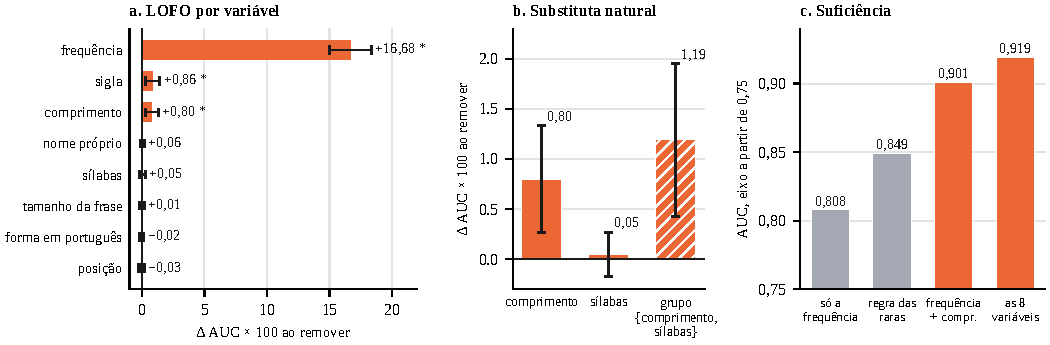
\includegraphics[width=\textwidth]{figuras/lofo_leitura.pdf}
\caption{LOFO na leitura, CompLex, com o mesmo protocolo da escrita e 50 dobras
agrupadas por palavra. a. Queda da AUC do Random Forest, em pontos de AUC
multiplicada por 100, ao remover cada variável, com intervalo de 95\%
corrigido; $^\ast p < 0,05$. b. Comprimento e sílabas, com $r = 0,87$, dividem a
importância; removidas juntas, a perda aparece. c. A frequência sozinha não
basta: fica abaixo da regra das palavras raras, e só com o comprimento se
aproxima do modelo completo.}
\label{fig:lofo_leitura}
\end{figure*}

As ordenações de importância do LOFO e da permutação, nas mesmas dobras,
tiveram correlação de Spearman de $\rho = 0,89$ na escrita, com intervalo de
95\% de 0,71 a 1,00, e de $\rho = 0,79$ na leitura, de 0,67 a 0,86. Os dois
métodos concordam no principal: o tempo de voo, na escrita, e a frequência, na
leitura. Na leitura, a permutação dá mais peso relativo a comprimento e sigla e
ainda destaca variáveis que o LOFO zera, como nome próprio e forma em
português.

\subsection{Escrita e leitura lado a lado}

A Tabela~\ref{tab:comparacao} reúne as duas tarefas. Como as variáveis de cada
base são diferentes, a variável dominante também é: o tempo de voo na escrita e
a frequência na leitura. Cada uma domina por um motivo direto. Na escrita, a
hesitação é a mediana da pausa entre teclas no texto livre, e o tempo de voo é a
mesma pausa medida na senha, isto é, o mesmo hábito de digitação observado em
outra tarefa. Na leitura, a frequência mede quanto a palavra aparece no idioma,
e as palavras raras são as que o leitor viu menos vezes; só ordenar os termos
pela raridade já dá AUC de 0,849.

O que se repete é o padrão: nas duas bases, o modelo interpretável alcança a
caixa-preta, a floresta é quase aditiva, uma variável concentra a informação e
a importância se divide quando há uma substituta. O que muda é a suficiência:
na escrita, o tempo de voo sozinho basta, e na leitura a frequência precisa do
comprimento. A base maior também permite distinguir efeitos menores. Na
leitura, sigla e comprimento, com menos de 1\% da AUC, seguem significativos
após a correção de Holm, enquanto na escrita o CV do tempo total, com 1,5\% do
RMSE, não se distingue de zero.

\begin{table}[!t]
\caption{Escrita e leitura lado a lado, com o mesmo protocolo.}
\label{tab:comparacao}
\centering
\footnotesize
\setlength{\tabcolsep}{4pt}
\begin{tabular}{@{}>{\raggedright\arraybackslash}p{1.7cm}
                >{\raggedright\arraybackslash}p{3.15cm}
                >{\raggedright\arraybackslash}p{3.15cm}@{}}
\toprule
 & \textbf{Escrita · KeyRecs} & \textbf{Leitura · CompLex} \\
\midrule
Tamanho          & 96 participantes, 7 variáveis & 8.579 termos, 8 variáveis \\
Interpretável    & Linear: RMSE de 0,0314~s, contra 0,0342~s da floresta, $p = 0,33$ & EBM: AUC de 0,919, igual à floresta, $p = 0,82$ \\
Aditividade      & Efeitos principais: \Rdois{}~$= 0,97$ & Efeitos principais: \Rdois{}~$= 0,93$ \\
Domina o LOFO    & Tempo de voo: +10,4~ms, 30\% do RMSE & Frequência: +16,7 pontos de AUC \\
Por que domina   & É a mesma pausa do alvo, medida na senha & Palavra rara é a que o leitor menos viu \\
Outras após Holm & Nenhuma & Sigla, +0,9, e comprimento, +0,8 \\
Basta sozinha    & Sim: 34,8 contra 34,6~ms & Não: 0,808; com o comprimento, 0,901 \\
Substituta       & Tempo total, de propósito, $r = 0,78$ & Sílabas, natural, $r = 0,87$ \\
Concordância     & $\rho = 0,89$ com a permutação, IC de 0,71 a 1,00 & $\rho = 0,79$ com a permutação, IC de 0,67 a 0,86 \\
\bottomrule
\multicolumn{3}{@{}p{0.97\columnwidth}@{}}{\scriptsize IC: intervalo de 95\%
por bootstrap das 10 repetições da validação cruzada.}
\end{tabular}
\end{table}

\begin{table*}[!t]
\caption{Síntese dos sete métodos globais aplicados ao Random Forest nas duas tarefas.}
\label{tab:sintese}
\centering
\footnotesize
\setlength{\tabcolsep}{5pt}
\renewcommand{\arraystretch}{1.12}
\begin{tabular}{@{}>{\raggedright\arraybackslash}p{3.3cm}
                >{\raggedright\arraybackslash}p{6.4cm}
                >{\raggedright\arraybackslash}p{6.6cm}@{}}
\toprule
\textbf{Método} & \textbf{Escrita · KeyRecs} & \textbf{Leitura · CompLex} \\
\midrule
H de Friedman
  & Mais interação: CV do tempo total e tempo de voo, $H = 0,17$ e 0,16, que formam o único par com interação
  & Mais interação: frequência, $H = 0,26$; par relevante mais forte: comprimento e sigla, $H = 0,27$ \\
Decomposição funcional
  & Efeitos principais: \Rdois{} $= 0,97$; interações: 3\%
  & Efeitos principais: \Rdois{} $= 0,93$; interações: 7\% \\
Permutação
  & Importa: tempo de voo, 17,4~ms; 6 de 7 sem efeito distinguível
  & Importam: frequência, comprimento, sigla; 3 com efeito mínimo; 2 sem efeito \\
Remoção, LOFO
  & Piora com $p < 0,05$, também após Holm: só o tempo de voo, +10,4~ms ou 30\% do RMSE, 1º nas 5 partições, que sozinho basta; $\rho = 0,89$ com a permutação
  & Piora com $p < 0,05$, também após Holm: frequência, +16,7 pontos de AUC, sigla e comprimento, +0,9 e +0,8; $\rho = 0,79$ \\
Substitutos globais
  & Árvore: \Rdois{} $= 0,98$; linear: \Rdois{} $= -0,38$; 1ª divisão: voo $\leq 0,138$
  & Árvore: \Rdois{} $= 0,91$; linear: \Rdois{} $= 0,79$; 1ª divisão: frequência $\leq 3,38$ \\
Extração de regras
  & 5 regras e SENÃO; fidelidade \Rdois{} $= 0,90$
  & 5 regras e SENÃO; fidelidade \Rdois{} $= 0,79$ \\
Protótipos e críticas
  & Críticas: maior voo e maior hesitação da amostra, um canhoto de 41 anos; erro médio de 0,043~s, contra 0,033~s nos protótipos
  & Críticas: siglas, nome próprio raro, palavra muito longa; probabilidade média de 0,50, contra 0,41 nos protótipos \\
\bottomrule
\end{tabular}
\end{table*}

\subsection{Resumos legíveis do Random Forest}

A Fig.~\ref{fig:fidelidade} compara a fidelidade dos resumos interpretáveis.
Uma árvore substituta de profundidade 3 reproduz o \RF{} com \Rdois{} de 0,98
na escrita e de 0,91 na leitura. A primeira divisão é tempo de voo
$\leq 0,138$~s na escrita, o mesmo corte da árvore podada da
Tabela~\ref{tab:escrita}, e frequência $\leq 3,38$ na leitura, seguida de
comprimento e sigla. A regressão linear substituta foi bem pior na escrita do
que na leitura, onde chegou a 0,79: nos 29 participantes de teste, seu \Rdois{}
foi negativo, de $-0,38$, isto é, pior do que prever a média, porque a reta
continua subindo onde a floresta se estabiliza.

\begin{figure}[!t]
\centering
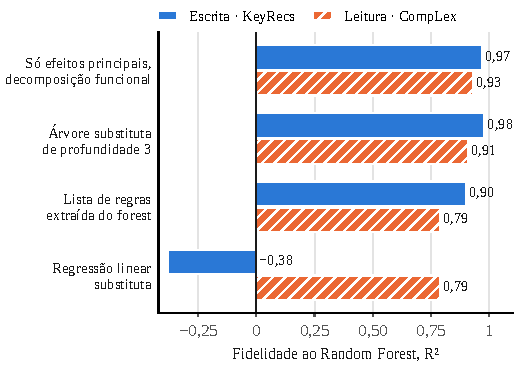
\includegraphics[width=\columnwidth]{figuras/fidelidade.pdf}
\caption{Fidelidade ao Random Forest de cada resumo interpretável, medida pelo
\Rdois{} entre as previsões do resumo e as do Random Forest no conjunto de
teste. Os efeitos principais, a árvore substituta e a lista de regras
reproduzem entre 79\% e 98\% da previsão; a regressão linear substituta fica
atrás e, na escrita, é pior do que prever a média.}
\label{fig:fidelidade}
\end{figure}

A lista de regras foi extraída dos caminhos de até duas condições das 500
árvores do \RF{}, escolhendo a cada passo a regra mais homogênea que cobre ao
menos 5\% dos casos restantes, até que uma nova regra acrescente menos de 0,01
à fidelidade no treino. Ela teve fidelidade de 0,90 na escrita e de 0,79 na
leitura, com 5 regras e SENÃO em cada uma. A Tabela~\ref{tab:regras} mostra as
duas primeiras regras e a regra SENÃO de cada lista. Elas repetem o que os
modelos interpretáveis já mostravam: tempo de voo acima de 0,14~s, na escrita,
e, na leitura, palavras frequentes que não são siglas, com probabilidade baixa,
deixando as raras e as siglas para o SENÃO.

\begin{table}[!t]
\caption{Primeiras regras extraídas do Random Forest.}
\label{tab:regras}
\centering
\footnotesize
\setlength{\tabcolsep}{4pt}
\begin{tabular}{@{}l>{\raggedright\arraybackslash}p{4.3cm}cc@{}}
\toprule
\textbf{Base} & \textbf{Regra} & \textbf{Previsão} & \textbf{Casos} \\
\midrule
Escrita & SE tempo de voo $> 0,143$                            & 0,121~s & 34\% \\
        & SE tempo de voo $\leq 0,130$ E CV do tempo total $> 0,389$ & 0,076~s & 25\% \\
        & mais 3 regras e SENÃO                                 & 0,082~s & 11\% \\
\midrule
Leitura & SE frequência $> 3,48$ E sílabas $\geq 2$              & 0,012   & 51\% \\
        & SE frequência $> 3,48$ E não é sigla                    & 0,022   & 18\% \\
        & mais 3 regras e SENÃO                                 & 0,420   & 13\% \\
\bottomrule
\multicolumn{4}{@{}p{0.95\columnwidth}@{}}{\scriptsize Escrita: hesitação
prevista, em s. Leitura: probabilidade prevista de o termo ser difícil. Casos:
proporção dos casos que caem em cada regra.}
\end{tabular}
\end{table}

\subsection{Casos típicos e atípicos}

O MMD-critic usou as variáveis padronizadas e um núcleo gaussiano, com largura
dada pela mediana das distâncias. O comportamento do modelo foi medido com
previsões fora da amostra, em validação cruzada de 5 dobras.

Na escrita, aplicado aos 96 participantes, o MMD-critic escolheu como
protótipos p012, p027, p083 e p075, destros de 21 a 25 anos com tempo de voo
entre 0,06 e 0,13~s, e como críticas p054, p077, p045 e p041. Entre as críticas
estão a participante com o maior tempo de voo e a maior hesitação da amostra,
p041, com 0,48 e 0,24~s, e um canhoto de 41 anos, p077, perfis raros entre os
96. O erro médio do modelo foi maior nas críticas, 0,043~s, do que nos
protótipos, 0,033~s: ele erra mais justamente onde os dados fogem do padrão.

Na leitura, o MMD-critic foi aplicado aos 832 termos difíceis. Os protótipos
foram \emph{alleles}, \emph{Spector}, \emph{CF}, \emph{earnestness},
\emph{mammon} e \emph{expiry}, termos típicos dos três corpora, na maioria
raros, e as críticas foram \emph{allele}, \emph{VIS}, \emph{CH}, \emph{Pinon},
\emph{totalitarianism} e \emph{SYN}: três siglas, um nome próprio raro e uma
palavra muito longa, em frases de até 137 palavras. O modelo atribuiu a elas
probabilidade média de 0,50, maior que a dos protótipos, 0,41, e a da média dos
termos difíceis, 0,36: esses casos atípicos são reconhecidos. Os termos que o
modelo mais deixa passar são outros: palavras comuns que os leitores acharam
difíceis, como \emph{season}, \emph{search} e \emph{matrix}, todas com
probabilidade abaixo de 0,01.

% =====================================================================
\section{Discussão}

\emph{Desempenho e explicabilidade.} Um bom desempenho preditivo não garante uma
boa explicação, e um empate entre modelos não implica que eles aprenderam a
mesma coisa. Aqui, os métodos globais mostram por que o empate ocorreu: o \RF{}
é quase aditivo nas duas tarefas, e um modelo aditivo, como a regressão ou o
EBM, consegue representar a maior parte do que ele aprendeu. O empate aparece em
todas as métricas da leitura, inclusive na precisão média, que é a mais
exigente para uma classe rara, e no Brier, que mede a calibração. Nesse
cenário, a recomendação de Rudin~\cite{rudin2019stop} se aplica: os modelos
interpretáveis por construção bastam.

\emph{Fidelidade não é verdade.} As fidelidades de 0,79 a 0,98 dizem quanto o
substituto ou a lista de regras se parece com o \RF{}, e não com o fenômeno. Um
resumo fiel de um modelo errado continua errado. Na escrita, a regressão linear
imita mal o \RF{}, com \Rdois{} de $-0,38$ no teste, embora seja o modelo com
menor erro preditivo. Isso é compatível com o degrau que o \RF{} aprende no
tempo de voo, perto de 0,14~s: uma estrutura que uma reta não reproduz, mas que
não se traduziu em ganho preditivo.

\emph{Correlação entre variáveis.} Comprimento e número de sílabas carregam
quase a mesma informação, com $r = 0,87$. Por isso, a remoção das sílabas não
prejudica o modelo, a do comprimento prejudica pouco, e só a remoção conjunta
mostra o peso do tamanho da palavra. A concordância menor entre permutação e
LOFO na leitura, com $\rho = 0,79$ contra 0,89 na escrita, é coerente com
variáveis correlacionadas, que dividem ou trocam a importância conforme o
método. Na permutação, nome próprio, tamanho da frase e forma em português
foram significativos com efeitos abaixo de 0,25 ponto de AUC: significância
estatística sem relevância prática. Na escrita, o experimento com o tempo total
da senha reproduz o fenômeno das substitutas de forma controlada, e a leitura o
mostra numa substituta natural.

\emph{Remover ou permutar.} LOFO, permutação e SHAP são explicações por
remoção, que diferem na forma de retirar a variável~\cite{covert2021explaining}.
A permutação mede quanto o modelo já treinado depende da variável, mas cria
combinações de valores que não existem nos dados e força o modelo a
extrapolar~\cite{hooker2021permutation}. O LOFO usa apenas dados reais, mas
explica o par formado pelo algoritmo e pelos dados, e não o modelo implantado.
O experimento com a variável substituta mostra a consequência prática: o LOFO
divide a importância entre as duas e poderia sugerir que nenhuma importa,
enquanto a permutação cai bem menos e continua apontando o tempo de voo. As duas
respostas estão certas, porque respondem a perguntas diferentes. Medida num
único corte de 30\% dos dados, a permutação parecia não mudar, de 18,6 para
18,3~ms; nas mesmas 50 dobras do LOFO, a queda aparece, o que mostra a vantagem
de calcular os dois métodos sobre as mesmas partições. Por isso, recomenda-se
relatar os dois métodos juntos, agrupar variáveis substitutas antes de concluir
que algo não importa e tratar a discordância entre eles como diagnóstico, e não
como erro.

\emph{O que o LOFO explica.} O LOFO muda com o algoritmo: o tempo de voo
responde por 30\% do RMSE na floresta e por 40\% na regressão linear. Muitos
modelos igualmente bons podem depender de variáveis
diferentes~\cite{fisher2019all}; para uma importância que não dependa do
algoritmo, Williamson et al.~\cite{williamson2023general} propõem uma versão
populacional, com inferência. Além disso, remover uma variável tira seu efeito
principal e todas as interações que a envolvem, como um efeito total. Isso ajuda
a ler o resultado do tempo de voo, que é também uma das variáveis com mais
interação, com $H = 0,16$. Um LOFO negativo, como o do pressionamento, indica
que o algoritmo generaliza melhor sem a variável nesta amostra, o que costuma
ser sobreajuste, e não uma afirmação sobre o fenômeno. Com vários testes ao
mesmo tempo, a correção de Holm evita que algum efeito pequeno pareça
significativo por acaso; aqui, os mesmos efeitos continuaram significativos
depois dela. O LOFO diz \emph{quanto} uma variável importa, mas não \emph{como}
nem por quê: a direção do efeito vem de métodos como PDP e ALE, e nenhuma
dessas medidas é causal.

\emph{Local e global.} Na escrita, as explicações locais da Atividade 03, LIME e
SHAP, a árvore podada, a árvore substituta e as regras apontam o mesmo limiar:
tempo de voo perto de 0,14~s. Na leitura, a árvore substituta e as regras
apontam palavras raras, abaixo de cerca de 3,4 na escala Zipf, e siglas. Essa
convergência entre métodos com hipóteses diferentes aumenta a confiança nas
conclusões, sem substituir uma validação com usuários.

\emph{Casos atípicos.} Nas duas tarefas, as críticas mostram perfis raros, mas
com consequências diferentes. Na escrita, o modelo erra mais nelas, sobretudo
na participante com o maior tempo de voo da amostra, e a amostra tem só 8
canhotos, o que pede cautela com a ausência de efeito da lateralidade. Na
leitura, as críticas, como siglas e palavras muito longas, são bem
reconhecidas, e as falhas estão em outro lugar: em palavras comuns que os
leitores acharam difíceis. Em \emph{matrix}, na expressão \emph{mitochondrial
matrix}, a dificuldade vem do sentido técnico da palavra no contexto, algo que
as variáveis atuais não capturam.

\emph{Limitações.} Na escrita, são 96 participantes em uma tarefa de
transcrição, e os métodos que usam um único conjunto de teste, como os
substitutos e as regras, contam com só 29 participantes. Na leitura, o termo
difícil é uma aproximação da busca real e está em inglês, e as variáveis foram
calculadas por nós: a frequência vem de uma lista externa, e sigla, nome
próprio e forma em português são regras simples sobre a grafia. O H de Friedman
é instável quando o efeito das variáveis é pequeno, e o H e as regras extraídas
dependem da amostra e podem variar com outra partição dos dados; no LOFO, só o
topo do ranking se mostrou estável. Ao treinar de novo sem cada variável, os
hiperparâmetros foram mantidos, e reajustá-los levou aos mesmos valores; mas
eles foram escolhidos em 70\% dos dados, que reaparecem como teste nas dobras,
o que pode deixar o erro de referência um pouco otimista. Uma validação
aninhada resolveria isso.

% =====================================================================
\section{Conclusão}

O objetivo foi verificar se modelos interpretáveis por construção bastam para
prever a hesitação na escrita e os termos difíceis na leitura, e entender o que
a caixa-preta aprendeu. Nas duas tarefas, o interpretável bastou: na escrita, a
regressão linear teve o menor erro, com RMSE de 0,031~s, sem diferença para o
\RF{}, $p = 0,33$; na leitura, o EBM igualou o \RF{} em AUC, de 0,919, em
precisão média e em calibração.

A principal evolução em relação às Atividades 02 a 04 foi levar o mesmo
protocolo a uma base nova, pública e bem maior. Isso permitiu separar o que é
próprio de cada tarefa, como a variável que domina e se ela basta sozinha, do
que se repete nas duas, e a base maior mostrou efeitos pequenos que a base da
escrita, com 96 participantes, não consegue distinguir de zero.

Os métodos globais mostraram que o \RF{} é quase aditivo, com 93\% a 97\% da
previsão vindo dos efeitos principais; que poucas variáveis concentram o
efeito; e que a árvore substituta e as regras o resumem com fidelidade de 0,79
a 0,98. O LOFO, com o mesmo protocolo nas duas bases, mostrou o mesmo padrão:
uma variável domina. Na escrita, é o tempo de voo na senha, com +10,4~ms no
RMSE, estável em todas as partições e nas versões da tabela; na leitura, é a
frequência, com +16,7 pontos de AUC. Na escrita, ela sozinha basta; na
leitura, precisa do comprimento. Nas duas, a importância se divide quando há
uma variável substituta, colocada de propósito na escrita e natural na leitura:
agrupar antes de descartar e comparar com a permutação são cuidados
necessários. Os casos atípicos indicam o que falta ao modelo de leitura:
reconhecer palavras comuns que são difíceis no contexto em que aparecem.

Como continuidade, pretendemos estender a leitura ao português e incluir
representações do termo no contexto, como vetores do E5~\cite{wang2024me5};
descer da pessoa para a palavra, usando a pausa antes de cada palavra no texto
livre da KeyRecs; e levar os modelos a um assistente pessoal proativo, híbrido
e multilíngue, que use as buscas salvas e a digitação das perguntas do
usuário. No LOFO, ainda cabem a importância populacional, com intervalo que não
depende do algoritmo~\cite{williamson2023general}; a validação aninhada; a
previsão da hesitação de uma sessão a partir da senha da outra; e medidas
baseadas em valores de Shapley, que repartem a importância entre variáveis
substitutas~\cite{covert2021explaining}.

% =====================================================================
\section*{Disponibilidade de dados e código}

Todo o trabalho, das Atividades 02 a 04 até esta etapa, está consolidado em um
único repositório, com os códigos, as tabelas, os resultados e uma cópia de cada
base, o que permite acompanhar a evolução do trabalho:
\url{https://github.com/deborazanoello/xai_identificacao_de_dificuldades_de_leitura_e_escrita}.
As duas bases são públicas e têm licença CC BY. A KeyRecs tem a fonte original
no Zenodo, \url{https://doi.org/10.5281/zenodo.7886743}, e a cópia em
\url{https://github.com/deborazanoello/xai_identificacao_de_dificuldades_de_leitura_e_escrita/tree/main/dados/keyrecs}.
O CompLex tem a fonte original no GitHub,
\url{https://github.com/MMU-TDMLab/CompLex}, e a cópia em
\url{https://github.com/deborazanoello/xai_identificacao_de_dificuldades_de_leitura_e_escrita/tree/main/dados/complex}.

% =====================================================================
\balance
\bibliographystyle{IEEEtran}
\bibliography{referencias}

\end{document}
